
%====================================================================================	
\section{Evaluation}

\begin{frame}{Evaluation}
	\begin{block}{Usability Tests}
		\begin{itemize}
			\item To understand if the application interface is well designed and perceptible. \\
		\end{itemize}
	\end{block}
	\begin{block}{Qualitative Tests}
			\begin{itemize}
				\item To gather users opinions. \\
			\end{itemize}
	\end{block}
	\begin{block}{Indicators Rating}
			\begin{itemize}
				\item To realize which indicators are the most convenient to any specific users. \\
			\end{itemize}
	\end{block}
	\begin{block}{Performance Tests}
			\begin{itemize}
				\item To verify the transactions costs. \\
			\end{itemize}
	\end{block}

\end{frame}
\note[itemize]{
\item la
\begin{block}{Usability Tests}
		\begin{itemize}
			\item Para perceber se a interface está bem desenhada e compreensivel
		\end{itemize}
	\end{block}
	\begin{block}{Qualitative Tests}
			\begin{itemize}
				\item Para colher as diferentes opiniões dos utilizadores relativamente à aplicação
			\end{itemize}
	\end{block}
	\begin{block}{Indicators Rating}
			\begin{itemize}
				\item A aplicação vai ter um sistema de rating de indicadores, onde os utilizadores poderão ajudar na selecção dos mesmos
			\end{itemize}
	\end{block}
	\begin{block}{Performance Tests}
			\begin{itemize}
				\item Para verificar os custos por transacção
			\end{itemize}
	\end{block}
}

\begin{frame}{Planning}

\begin{figure}
  \centering
  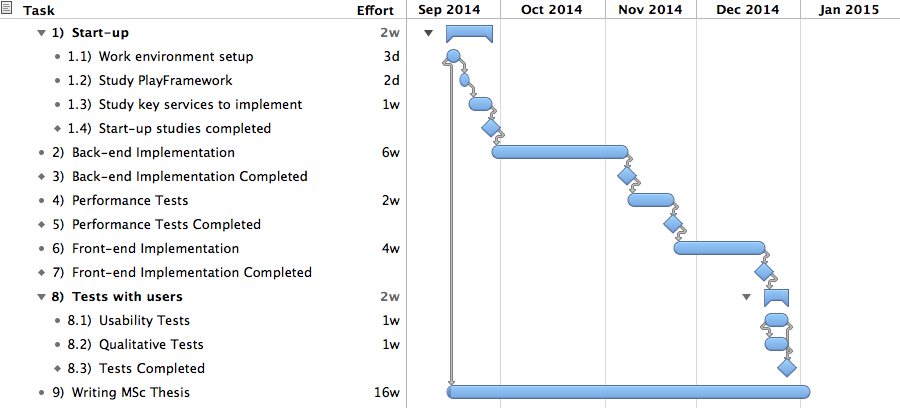
\includegraphics[width=1\textwidth]{images/PlaneamentoTese.png}
  \label{fig:PlaneamentoTese}
\end{figure}

\end{frame}
\note[itemize]{
\item Esta tese tem de ser entregue no inicio de Janeiro,
\item Estou a contar terminá-la antes do final de Dezembro já devido às festas do Natal e Passagem de Ano
\item O trabalho vai começar por um set-up do sistema para desenvolvimento, seguido do desenvolvimento de back-end e só depois do fron-end e interface do sistema.
\item Por fim, serão realizados os diferentes testes aos utilizadores.
}